%!TEX TS-program = xelatex
\documentclass[a4paper, 12pt]{article}
\usepackage{barinovxesimple}
\geometry{top=25mm}
\geometry{bottom=35mm}
\geometry{left=35mm}
\geometry{right=20mm}
\setlist{labelindent=\parindent,leftmargin=*}
\begin{document}
\thispagestyle{empty}
\begin{center}
    \textit{Федеральное государственное автономное образовательное\\ учреждение высшего образования }

    \vspace{0.5ex}

        \textbf{«Московский физико-технический институт\\ (национальный исследовательский университет)»}
\end{center}

\vspace{10ex}

\begin{center}
    \vspace{13ex}

    \so{\textbf{Лабораторная работа №-.-.-}}

    \vspace{1ex}

    по курсу общей физики

    на тему:

    \textbf{\textit{<<>>}}

    \vspace{30ex}

    \begin{flushright}
        \noindent
        \textit{Работу выполнил:}\\  
        \textit{Баринов Леонид \\(группа Б02-827)}
    \end{flushright}
    \vfill
    Долгопрудный \\2019
\newpage
\setcounter{page}{1}
\fancyhead[R]{\nouppercase{\leftmark}}	
\end{center}

\section{Аннотация}
В работе будет исследована температурная зависимость проводимости
типичного полупроводника и меди, определена ширина
запрещенной зоны полупроводника с помощью универсального цифрового
вольтметра В7-34А.






\section{Теоретические сведения}

Величина электропроводности в полупроводниках определяется числом
электронов в зоне проводимости и дырок в валентной зоне. Число электронов, находящихся в зоне проводимости, равно произведению
числа имеющихся уровней на вероятность их заполнения. 

Вероятность заполнения уровней определяется функцией Ферми
\begin{equation}
    f(E) = \frac{1}{\exp \left(\dfrac{E-\mu}{k_{Б}T}\right)+1} \approx
    \exp \left(- \frac{E-\mu}{k_{Б}T}\right)\hspace{1em} \left( при\: (E-\mu)\gg
    k_{Б}T \right)
    \label{eq:1}
\end{equation}
$\mu$ --- уровень Ферми. 

Число электронов в зоне проводимости будет равно 
\begin{equation}
    n_{n} = Q_{n} \exp \left( -\frac{E_{c}-\mu}{k_{Б}T}\right)
    \label{eq:2}
\end{equation}
$E_{c}$ --- энергия дна зоны проводимости, $Q_{n}$ --- эффективное
число уровней, находящихся вблизи дна зоны.

Число дырок в зоне проводимости будет равно 
\begin{equation}
    n_{p} = Q_{p} \exp \left( -\frac{E_{v}-\mu}{k_{Б}T}\right)
    \label{eq:2}
\end{equation}
$E_{v}$ --- энергия верхнего края валентной зоны, $Q_{p}$ --- эффективное
число уровней, находящихся вблизи края валентной зоны.

Для проводника без примесей число электронов будет равно числу дырок,
тогда

\begin{equation}
    n_{n}n_{p} = n^2 = Q_{n}Q_{p} \exp \left(-
    \frac{E_{c}-E_{v}}{k_{Б}T}\right)
    \label{eq:3}
\end{equation}


Выражая $n$ и обозначая $C = \sqrt{Q_{n}Q_{p}}$, а $E_{c}-E_{v} =
\Delta$ --- ширина запрещенной зоны, получаем
\begin{equation}
    n= C \exp \left(- \frac{\Delta}{2k_{Б}T}\right)
    \label{eq:4}
\end{equation}

Зависимость средней дрейфовой скорости электронов $v_{ср}$ от
напряженности электрического поля
\begin{equation}
    v_{ср}=\mu_{n}E
    \label{eq:5}
\end{equation}
$\mu_{n}$ --- коэффициент пропорциональности, носящий название
подвижности электронов.

Плотность электрического тока определяется по формуле $j = n e
v_{ср}$, тогда проводимость $\sigma$ будет равна 
\begin{equation}
    \sigma = j/E = e \left(n_{n} \mu_{n} + n_{p}\mu_{p}\right)
    \label{eq:6}
\end{equation}

Окончательно получим ($n_{n}=n_{p}$)
\begin{equation}
    \sigma = e C \left(\mu_{n} + \mu_{p}\right) \exp \left(-
    \frac{\Delta}{2k_{Б}T}\right) = A \exp \left(-
\frac{\Delta}{2k_{Б}T}\right)
    \label{eq:7}
\end{equation}



\section{Оборудование}
Для изучения зависимости $\sigma(T)$ используется установка,
схематически изображенная на \fig{fig:1}

\begin{figure}[H]
    \includegraphics[width=0.8\linewidth]{1} 
    \caption{Схема установки по измерению зависимости $\sigma(T)$ с
    помощью вольтметра В7-34А}
    \label{fig:1}
\end{figure}

Исследуемые образцы $(O_{1}$ и $O_{2})$ в специальном зажиме помещаются
в электронагревательную печь \textit{П}. Сопротивление образцов
измеряется универсальным цифровым вольтметром В7-34А, который
обеспечивает высокую точность измерений.

Удельная проводимость находится по формуле 
\begin{equation}
    \sigma = \frac{l}{RS}
    \label{eq:8}
\end{equation}
где $R$ --- сопротивление образца, $l$ --- его длина, $S$ ---
поперечное сечение образца. В нашем случае $l = 13,4\: м$, а $S = \pi
d^2/4 = 3,85\: мм^2$

\section{Результаты измерений и обработка результатов}

\newgeometry{left=22mm, right=20mm, top=25mm, bottom=35mm}

\renewcommand{\arraystretch}{1.1}
\begin{table}[H]
\centering
\begin{tabular}{|c|c|c|c|c|c|c|c|}
\hline
$U,\: мВ$ & $T,\: К$  & $R_{пп},\: Ом$ & $R_{Cu},\: Ом$ &
\begin{tabular}{c}$\sigma_{пп},$\\ $(Ом\cdot мм)^{-1}$\end{tabular}  &
\begin{tabular}{c}$\sigma_{Cu},$\\ $(Ом\cdot
мм)^{-1}$ \end{tabular}&
\begin{tabular}{c}$1/T,$ \\ $10^{-3} К^{-1}$\end{tabular}    & $\ln \sigma_{пп}$ \\ \hline
0,21  & 303,12 & 288,1   & 181,3   & 12,08  & 19,20 & 3,30 & 2,492  \\ \hline
0,21  & 303,12 & 287,9   & 181,4   & 12,09  & 19,19 & 3,30 & 2,492  \\ \hline
0,22  & 303,37 & 287,6   & 181,4   & 12,10  & 19,19 & 3,30 & 2,493  \\ \hline
0,24  & 303,85 & 287,2   & 181,5   & 12,12  & 19,18 & 3,29 & 2,495  \\ \hline
0,26  & 304,34 & 286,2   & 181,6   & 12,16  & 19,17 & 3,29 & 2,498  \\ \hline
0,30  & 305,32 & 283,8   & 181,9   & 12,26  & 19,13 & 3,28 & 2,507  \\ \hline
0,42  & 308,24 & 275,1   & 183,3   & 12,65  & 18,99 & 3,24 & 2,538  \\ \hline
0,50  & 310,20 & 266,8   & 184,4   & 13,05  & 18,87 & 3,22 & 2,568  \\ \hline
0,61  & 312,88 & 254,4   & 186,1   & 13,68  & 18,70 & 3,20 & 2,616  \\ \hline
0,75  & 316,29 & 237,7   & 188,2   & 14,64  & 18,49 & 3,16 & 2,684  \\ \hline
0,81  & 317,76 & 229,5   & 189,0   & 15,17  & 18,42 & 3,15 & 2,719  \\ \hline
0,97  & 321,66 & 206,4   & 191,6   & 16,86  & 18,17 & 3,11 & 2,825  \\ \hline
1,11  & 325,07 & 184,5   & 193,8   & 18,86  & 17,96 & 3,08 & 2,937  \\ \hline
1,24  & 328,24 & 169,0   & 195,8   & 20,59  & 17,78 & 3,05 & 3,025  \\ \hline
1,35  & 330,93 & 153,0   & 198,0   & 22,75  & 17,58 & 3,02 & 3,124  \\ \hline
1,52  & 335,07 & 133,0   & 200,6   & 26,17  & 17,35 & 2,98 & 3,265  \\ \hline
1,70  & 339,46 & 114,0   & 203,6   & 30,53  & 17,09 & 2,95 & 3,419  \\ \hline
1,85  & 343,12 & 101,0   & 206,0   & 34,46  & 16,90 & 2,91 & 3,540  \\ \hline
1,98  & 346,29 & 91,0    & 208,2   & 38,25  & 16,72 & 2,89 & 3,644  \\ \hline
2,18  & 351,17 & 77,0    & 211,4   & 45,20  & 16,46 & 2,85 & 3,811  \\ \hline
2,30  & 354,10 & 70,0    & 213,4   & 49,72  & 16,31 & 2,82 & 3,906  \\ \hline
2,40  & 356,54 & 65,0    & 215,0   & 53,55  & 16,19 & 2,80 & 3,981  \\ \hline
2,75  & 365,07 & 49,6    & 220,6   & 70,17  & 15,78 & 2,74 & 4,251  \\ \hline
2,92  & 369,22 & 44,0    & 223,3   & 79,10  & 15,59 & 2,71 & 4,371  \\ \hline
3,00  & 371,17 & 41,0    & 224,5   & 84,89  & 15,50 & 2,69 & 4,441  \\ \hline
3,09  & 373,37 & 38,9    & 226,0   & 89,47  & 15,40 & 2,68 & 4,494  \\ \hline
3,22  & 376,54 & 35,0    & 228,0   & 99,44  & 15,27 & 2,66 & 4,600  \\ \hline
3,35  & 379,71 & 32,2    & 230,3   & 108,09 & 15,11 & 2,63 & 4,683  \\ \hline
3,45  & 382,15 & 30,2    & 231,8   & 115,25 & 15,02 & 2,62 & 4,747  \\ \hline
3,57  & 385,07 & 28,0    & 233,6   & 124,30 & 14,90 & 2,60 & 4,823  \\ \hline
3,70  & 388,24 & 25,7    & 235,3   & 135,43 & 14,79 & 2,58 & 4,908  \\ \hline
3,79  & 390,44 & 24,1    & 237,1   & 144,42 & 14,68 & 2,56 & 4,973  \\ \hline
3,88  & 392,63 & 22,8    & 238,5   & 152,65 & 14,59 & 2,55 & 5,028  \\ \hline
\end{tabular}
\caption{Зависимость сопротивления меди $R_{Cu}$ и полупроводника
$R_{пп}$ от температуры $T,\: К$, определенной с помощью напряжения на
термопаре $U$}
\end{table}

\restoregeometry

Построим график зависимости удельной проводимости полупроводника и
меди $\sigma$ от температуры $T$.


\begin{figure}[H]
    \includegraphics[width=0.9\linewidth]{2} 
    \caption{График зависимости удельной проводимости полупроводника и
меди $\sigma$ от температуры $T$}
\label{fig:2}
\end{figure}

Построим график зависимости сопротивления меди $R_{Cu}$ от температуры
$T$


\begin{figure}[H]
    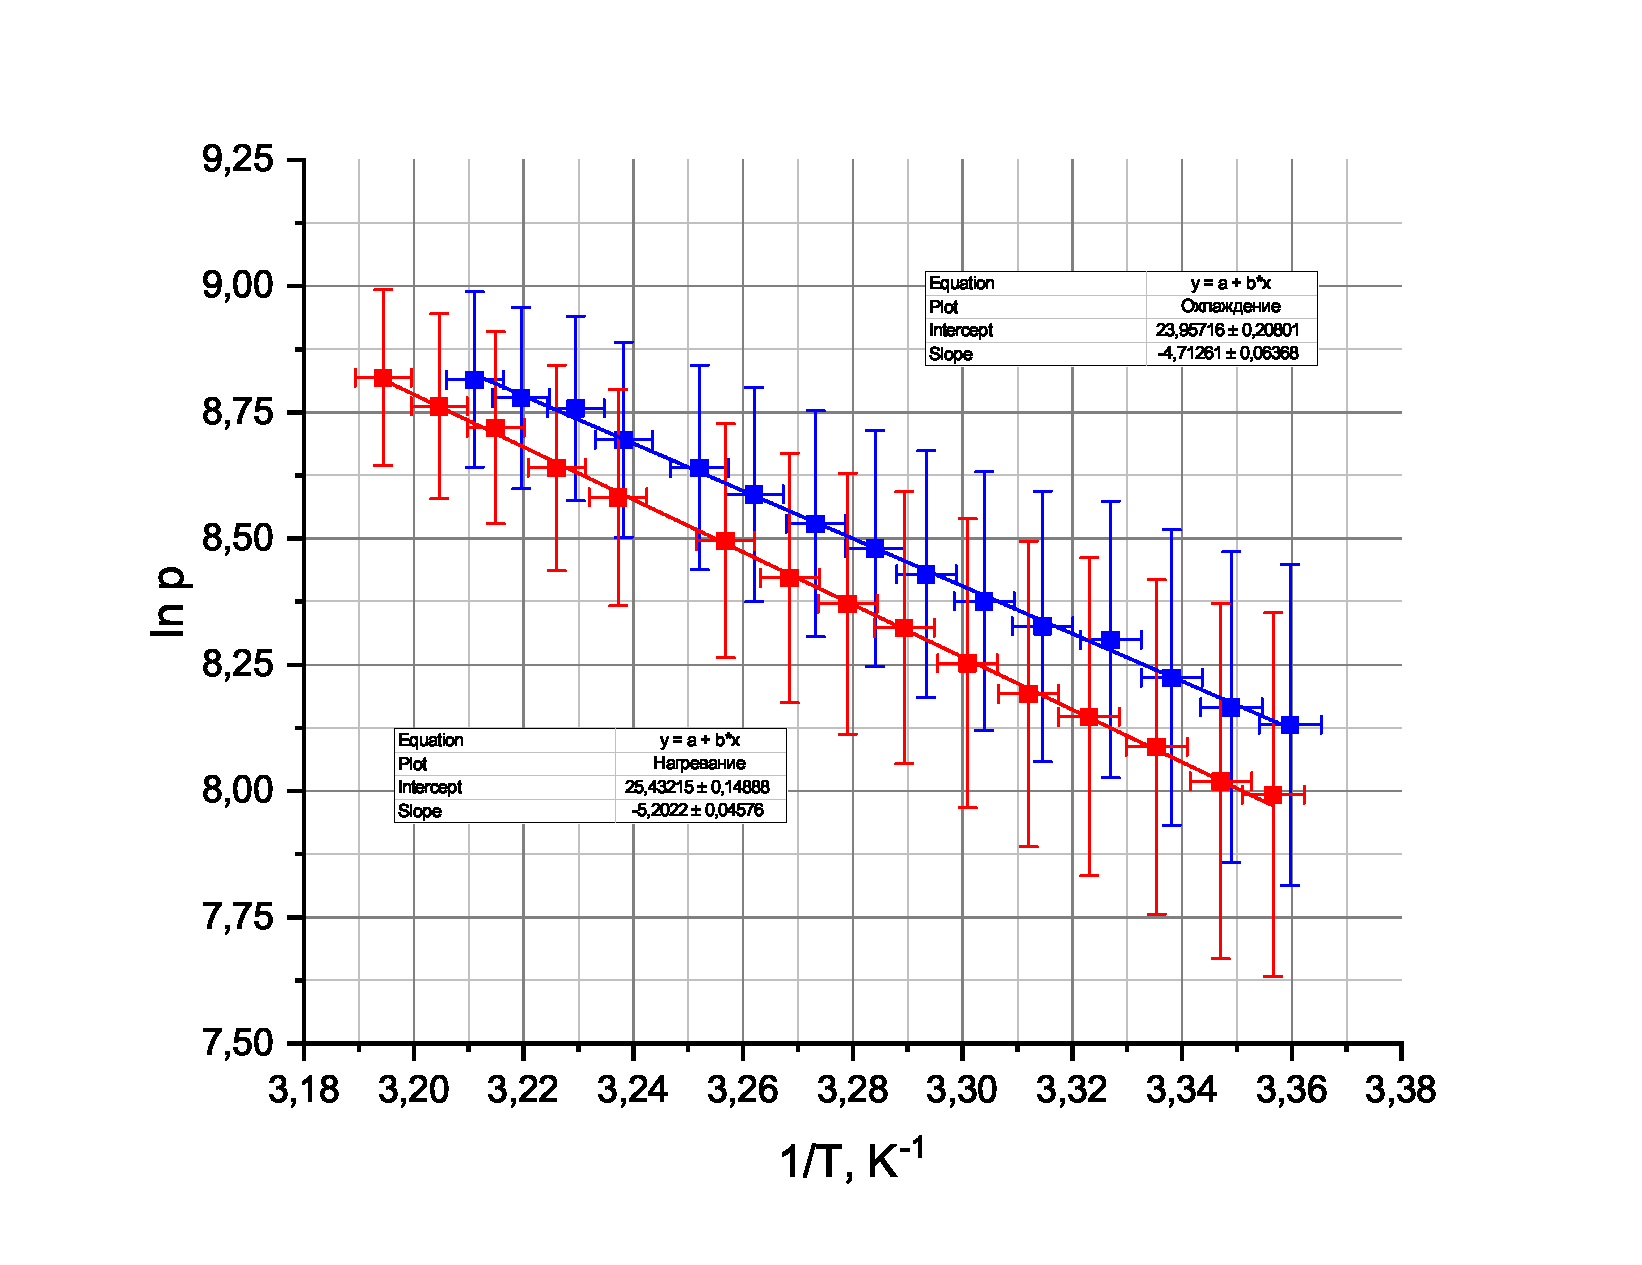
\includegraphics[width=0.9\linewidth]{4} 
    \caption{График зависимости сопротивления меди $R_{Cu}$ от температуры
$T$}
\label{fig:3}
\end{figure}

Коэффициент наклона равен 

\[
    k_{1} = (0,648 \pm 0,003)\: Ом/К
\]

Определим температурный коэффициент сопротивления меди:

\[
    \alpha = \dfrac{k_{1}}{R(T_{0})} = (35,7 \pm 0,2)\:10^{-4}\: К^{-1}
\]

Построим график зависимости $\ln \sigma$ от $1/T$ для полупроводника

\begin{figure}[H]
    \includegraphics[width=0.9\linewidth]{3} 
    \caption{График зависимости $\ln \sigma$ от $1/T$ для полупроводника}
    \label{fig:4}
\end{figure}


Коэффициент наклона равен 

\[
    k_{2} = (3,98 \pm 0,02)\: 10^{3}\: К^{-1}
\]

Определим запрещенную зону полупроводника:

\[
    \Delta = 2 k_{Б} k_{2} = (0,686 \pm 0,013)\: эВ
\]













\section{Обсуждение результатов и выводы}


В работе была исследована температурная зависимость проводимости
полупроводника и меди \ffig{fig:2}. По графику зависимости
сопротивления меди $R_{Cu}$ от температуры $T$ \ffig{fig:3} был
определен температурный коэффициент сопротивления меди
\[
    \alpha = (35,7 \pm 0,2)\:10^{-4}\: К^{-1}
\]

Значение довольно близко к табличному 
\[
    \alpha^т = 41\cdot 10^{-4}\: К^{-1}
\]

По графику зависимости логарифма проводимости $\ln \sigma$ от
температуры $T$ для полупроводника была найдена ширина запрещенной
зоны $\Delta$
\[
    \Delta = (0,686 \pm 0,013)\: эВ
\]

В пределах погрешности экспериментальное значение совпадет с шириной
запрещенной зоны германия:
\[
    \Delta_{\text{Ge}} = 0,67\: эВ
\]









\end{document}
